\section{Informationsverarbeitung}

\subsection{Digitalrechner}
\begin{figure}[H]
    \begin{center}
    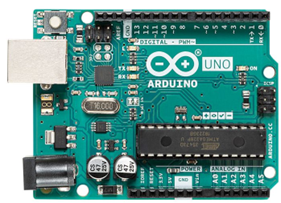
\includegraphics[width=7cm]{Digitalrechner_Arduino Uno.png}
    \end{center}
    \caption{Arduino}
\end{figure}

Auf dem Arduino ist ein Atmega328 Mikroprozessor verbaut. Dieser ist auf einer Platine beschaltet. Das Programm kann mit der Arduino IDE direkt über eine serielle Schnittstelle auf den Arduino geladen werden. Es wird also kein externes Kompiliergerät benötigt. Mit der Arduino IDE lassen sich auf dem Arduino UNO rund 20 Pins programmieren. Bei einem Arduino UNO sind folgende Anschlüsse vorhanden:

\begin{itemize}
    \item 13x digital Pins 
    \item 3x Timer 
    \item 6x PWM Pins 
    \item SDA und SCL Pins 
    \item 6x analog Pins 
    \item MISO MOSI Pins
\end{itemize}

Benutzt werden hierbei 5 der PWM-Pins, 4 der normalen Digital-Pins, die SDA- und SCL-Pins. Der USB-Anschluss wird lediglich zur Übertragung des Programms und zur Überwachung der korrekten Funktion während der Entwicklung benötigt.


\subsection{Steuerung}
Die Steuerung des Roboters erfolgt lediglich über die Motoren, welche mit unterschiedlichen PWM-Signalen neben vorwärtsn nach links und nach rechts gesteuert werden. 

\subsection{Regelung}
Die Regelung erfolgt über eine Kombination aus Kompass, den GPS-Koordinaten des Handys und den GPS-Koordinaten des GPS-Moduls, welches mit dem Arduino verbunden ist. Mittels der 2 Koordinatensets soll die Distanz zwischen den beiden Punkten errechnet werden, der Kompass gibt schliesslich die Richtung an, in welche es sich zu drehen gilt. Sobald die Distanz unter einen gewissen Schwellenwert fällt, wird die Position des Handy-GPS wieder überprüft und der Prozess beginnt von vorne. 
\\ \\
Das Fundament für die Berechnung bildet die Natur des GPS-Koordinatensystems. Dieses hat seinen «Nullpunkt» am Schnittpunkt zwischen Äquator und dem Null-Meridian, der Nord-Süd Achse durch Greenwich, Vereinigtes Königreich. 
Ein GPS-Standpunkt ist stets in Latitude und Longitude unterteilt. Die Latitude gibt den Winkel zwischen der Äquatorlinie und dem Standpunkt an und die Longitude gibt den Winkel zwischen Nullmeridian und dem Standpunkt an.
\\ \\
Dank der Haversine Formel 

\[a=sin^{2}\left ( \frac{p_{2}.lat-p_{1}.lat}{2} \right )+cos\left ( p_{1}.lat \right )*cos\left ( p_{2}.lat \right )*sin^{2}\left ( \frac{p_{2}.lon-p_{1}.lon}{2} \right )\]
\[b=2*atan2\left ( \sqrt{a},\sqrt{1-a} \right )\]
\[d=R*b\]

lässt sich die Distanz zwischen 2 GPS-Punkten relativ leicht berechnen. R ist der Erdradius von 6371 km. \\ \\
Über folgende Formel:

\[\beta = atan2(sin\left ( p_{2}.lon-p_{1}.lon \right )*cos\left ( p_{2}.lat \right ), cos\left (p_{1}.lat  \right )*sin\left ( p_{2}.lat \right )-\] 
\[sin\left ( p_{1}.lat \right )*cos\left (p_{2}.lat  \right )*cos\left ( p_{2}.lon-p_{1}.lon \right ))\]

lässt sich indes der Winkel zwischen der Nord-Süd-Achse durch Punkt 1 und der Achse, welche durch die beiden Punkte geht, berechnen. Man nennt dies die Peilrichtung, oder Bearing.
\\ \\
Wenn man nun den Winkel, resp. die eigene Ausrichtung gegenüber dem Nordpol kennt, zum Beispiel durch einen Kompass, kann man diesen Winkel von der Peilrichtung abziehen und erhält den Winkel, um den man sich drehen muss, um in Richtung des zweiten Punktes zu zeigen.
